\section{Introduction}

  This program demonstrates a method for normalizing a group of face images with hand labeled
features.  This normalization method attempts to map five points to a set of five predefined locations using an Affine transform.  Because each point consists of two parts (x and y) a total of 10 equations are known while the Affine transformation matrix only has 6 parameters.  This leads to an over-determined system which very likely has no solution.  By using a method known as Singular Value Decomposition(SVD), the solution which yields the least Mean Square Error(MSE) can be computed efficiently.

A method for correcting non-uniform illumination in the resulting face images was also implemented.  This method involves solving for the coefficients of Eq.~\ref{eq:1} with respect to every pixel in the image.  This means for an NxM image, there are 4 unknown and NM equations.  Because this system is also over-determined, SVD was used to calculate the least MSE coefficients. 

\begin{equation}
  \label{eq:1}
  f(x,y)=ax+by+cxy+d
\end{equation}

\section{Results}
  
  The results of the normalization process were very favorable (Fig. 1). While the points in the images could not be mapped exactly to the desired locations, Fig. 2 shows that the features were all very close.  The white circles have a radius of 5 pixels and the black circles have a radius of 4 pixels.  Fig. 2 shows that no feature was more than 9 pixels away from its desired position and in most cases the features were no more than 3 pixels away.

  The light correction function calculated using SVD can be seen in Fig. 3.  The final results of the light correction can be seen in Fig. 4.  While this method seemed to work well in most cases, it seemed to have trouble when a large amount of dark background was in an image.  The black background seemed to overpower the function and cause it to try and lighten this area while darkening bright area causing an odd shadowing effect.

\section{Conclusion}

  By implementing these methods I learned a great deal about using SVD for solving over-determined systems.  I also learned a great deal about Affine transforms and how to map the pixels using an inverse to ensure no holes are left in the transformed image.

  Originally I was confused about why an iterative method is used here rather than directly mapping each image to the final locations.  The reason I came up with is that this iterative method not only aligns the images to the final location but also to each other.  By using this iterative method even if the final location points are chosen poorly, all the faces should be mapped to approximately the same locations.

  The light correction part was also an interesting concept, it shows how a relatively simple function like Eq.~\ref{eq:1} can be used to correct major intensity inconsistencies in an image.

\newpage

\section{Images}
  %\begin{figure}[hbt]
%  \centering
%  \subfigure[CAP]{
%    \includegraphics[width=0.4\textwidth]{}
%  }
%  \caption{}
%  % Put the label at the bottom
%  \label{fig:}
%\end{figure}

\begin{figure}[hbt]
  \centering
  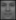
\includegraphics[width=0.25\textwidth]{../results/H_rez/mean_face.jpg}
  \caption{Average face}
  \label{fig:mean}
\end{figure}

~\vfill

\begin{figure}[hbt]
  \centering
  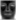
\includegraphics[width=0.18\textwidth]{../results/H_rez/eigenfaces/largest1.jpg}
  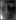
\includegraphics[width=0.18\textwidth]{../results/H_rez/eigenfaces/largest2.jpg}
  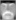
\includegraphics[width=0.18\textwidth]{../results/H_rez/eigenfaces/largest3.jpg}
  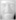
\includegraphics[width=0.18\textwidth]{../results/H_rez/eigenfaces/largest4.jpg}
  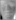
\includegraphics[width=0.18\textwidth]{../results/H_rez/eigenfaces/largest5.jpg} \\
  \vspace{4pt}
  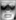
\includegraphics[width=0.18\textwidth]{../results/H_rez/eigenfaces/largest6.jpg}
  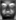
\includegraphics[width=0.18\textwidth]{../results/H_rez/eigenfaces/largest7.jpg}
  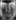
\includegraphics[width=0.18\textwidth]{../results/H_rez/eigenfaces/largest8.jpg}
  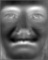
\includegraphics[width=0.18\textwidth]{../results/H_rez/eigenfaces/largest9.jpg}
  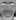
\includegraphics[width=0.18\textwidth]{../results/H_rez/eigenfaces/largest10.jpg}
  \caption{Top ten Eigenfaces}
  \label{fig:top_efaces}
\end{figure}

~\vfill

\begin{figure}[hbt]
  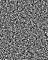
\includegraphics[width=0.09\textwidth]{../results/H_rez/eigenfaces/smallest1.jpg}
  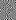
\includegraphics[width=0.09\textwidth]{../results/H_rez/eigenfaces/smallest2.jpg}
  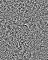
\includegraphics[width=0.09\textwidth]{../results/H_rez/eigenfaces/smallest3.jpg}
  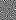
\includegraphics[width=0.09\textwidth]{../results/H_rez/eigenfaces/smallest4.jpg}
  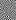
\includegraphics[width=0.09\textwidth]{../results/H_rez/eigenfaces/smallest5.jpg}
  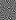
\includegraphics[width=0.09\textwidth]{../results/H_rez/eigenfaces/smallest6.jpg}
  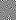
\includegraphics[width=0.09\textwidth]{../results/H_rez/eigenfaces/smallest7.jpg}
  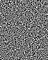
\includegraphics[width=0.09\textwidth]{../results/H_rez/eigenfaces/smallest8.jpg}
  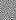
\includegraphics[width=0.09\textwidth]{../results/H_rez/eigenfaces/smallest9.jpg}
  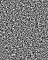
\includegraphics[width=0.09\textwidth]{../results/H_rez/eigenfaces/smallest10.jpg}
  \caption{Bottom ten Eigenfaces}
  \label{fig:bot_efaces}
\end{figure}

~\vfill

\vfill

~\vfill

\begin{figure}[hbt]
  \centering
  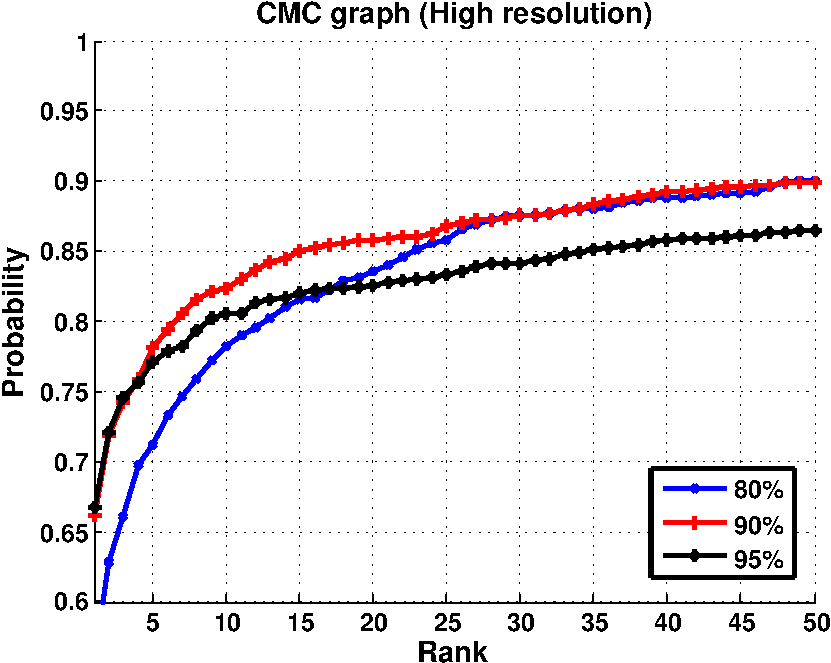
\includegraphics[width=0.7\textwidth]{../results/Output_H.pdf}
  \caption{High resolution CMC for training at 80\%, 90\%, and 95\% information retention.}
  \label{fig:cfc_h}
\end{figure}

~\vfill

\begin{figure}[hbt]
  \centering
  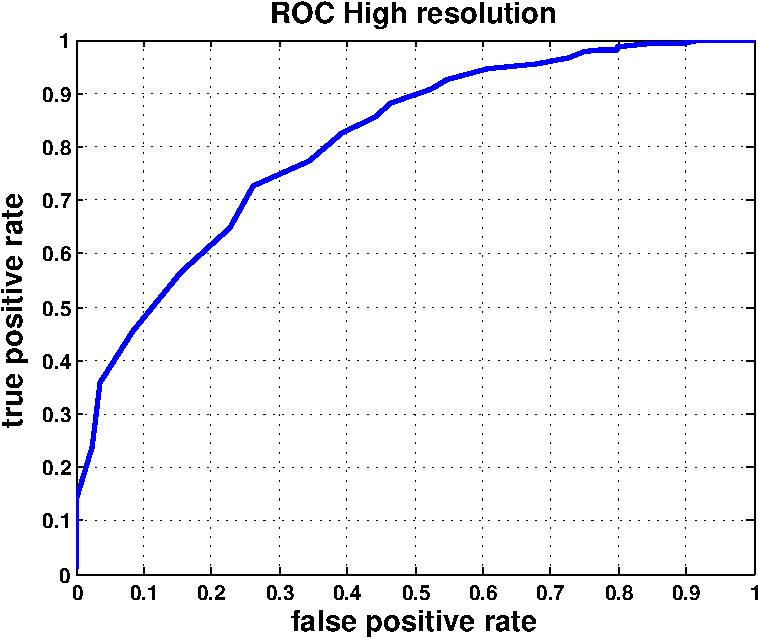
\includegraphics[width=0.7\textwidth]{../results/ROC_H.pdf}
  \caption{High resolution ROC.}
  \label{fig:roc_h}
\end{figure}

~\vfill

\vfill

~\vfill

\begin{figure}[hbt]
  \centering
  \includegraphics[width=0.1\textwidth]{../results/H_rez/correct80/1/testImg.jpg} \vline
  \hspace{2pt}
  \includegraphics[width=42pt]{../results/H_rez/correct80/1/1.jpg}
  \includegraphics[width=42pt]{../results/H_rez/correct80/1/2.jpg}
  \includegraphics[width=31pt]{../results/H_rez/correct80/1/3.jpg}
  \includegraphics[width=42pt]{../results/H_rez/correct80/1/4.jpg}
  \includegraphics[width=31pt]{../results/H_rez/correct80/1/5.jpg}
  \includegraphics[width=31pt]{../results/H_rez/correct80/1/6.jpg}
  \includegraphics[width=42pt]{../results/H_rez/correct80/1/7.jpg}
  \includegraphics[width=42pt]{../results/H_rez/correct80/1/8.jpg}
  \includegraphics[width=31pt]{../results/H_rez/correct80/1/9.jpg}
  \includegraphics[width=31pt]{../results/H_rez/correct80/1/10.jpg} \\
  \vspace{4pt}
  \includegraphics[width=0.1\textwidth]{../results/H_rez/correct80/2/testImg.jpg} \vline
  \hspace{2pt}
  \includegraphics[width=0.09\textwidth]{../results/H_rez/correct80/2/1.jpg}
  \includegraphics[width=0.09\textwidth]{../results/H_rez/correct80/2/2.jpg}
  \includegraphics[width=0.07\textwidth]{../results/H_rez/correct80/2/3.jpg}
  \includegraphics[width=0.09\textwidth]{../results/H_rez/correct80/2/4.jpg}
  \includegraphics[width=0.07\textwidth]{../results/H_rez/correct80/2/5.jpg}
  \includegraphics[width=0.09\textwidth]{../results/H_rez/correct80/2/6.jpg}
  \includegraphics[width=0.07\textwidth]{../results/H_rez/correct80/2/7.jpg}
  \includegraphics[width=0.07\textwidth]{../results/H_rez/correct80/2/8.jpg}
  \includegraphics[width=0.07\textwidth]{../results/H_rez/correct80/2/9.jpg}
  \includegraphics[width=0.07\textwidth]{../results/H_rez/correct80/2/10.jpg} \\
  \vspace{4pt}
  \includegraphics[width=0.1\textwidth]{../results/H_rez/correct80/3/testImg.jpg} \vline
  \hspace{2pt}
  \includegraphics[width=0.09\textwidth]{../results/H_rez/correct80/3/1.jpg}
  \includegraphics[width=0.07\textwidth]{../results/H_rez/correct80/3/2.jpg}
  \includegraphics[width=0.09\textwidth]{../results/H_rez/correct80/3/3.jpg}
  \includegraphics[width=0.07\textwidth]{../results/H_rez/correct80/3/4.jpg}
  \includegraphics[width=0.09\textwidth]{../results/H_rez/correct80/3/5.jpg}
  \includegraphics[width=0.07\textwidth]{../results/H_rez/correct80/3/6.jpg}
  \includegraphics[width=0.07\textwidth]{../results/H_rez/correct80/3/7.jpg}
  \includegraphics[width=0.07\textwidth]{../results/H_rez/correct80/3/8.jpg}
  \includegraphics[width=0.07\textwidth]{../results/H_rez/correct80/3/9.jpg}
  \includegraphics[width=0.09\textwidth]{../results/H_rez/correct80/3/10.jpg}
  \caption{Top matches for 3 correctly matched faces at 80\% information retention.}
  \label{fig:correct80}
\end{figure}

~\vfill

\begin{figure}[hbt]
  \centering
  \includegraphics[width=0.1\textwidth]{../results/H_rez/incorrect80/1/testImg.jpg} \vline
  \hspace{2pt}
  \includegraphics[width=0.08\textwidth]{../results/H_rez/incorrect80/1/1.jpg}
  \includegraphics[width=0.08\textwidth]{../results/H_rez/incorrect80/1/2.jpg}
  \includegraphics[width=0.08\textwidth]{../results/H_rez/incorrect80/1/3.jpg}
  \includegraphics[width=0.08\textwidth]{../results/H_rez/incorrect80/1/4.jpg}
  \includegraphics[width=0.08\textwidth]{../results/H_rez/incorrect80/1/5.jpg}
  \includegraphics[width=0.08\textwidth]{../results/H_rez/incorrect80/1/6.jpg}
  \includegraphics[width=0.08\textwidth]{../results/H_rez/incorrect80/1/7.jpg}
  \includegraphics[width=0.08\textwidth]{../results/H_rez/incorrect80/1/8.jpg}
  \includegraphics[width=0.08\textwidth]{../results/H_rez/incorrect80/1/9.jpg}
  \includegraphics[width=0.08\textwidth]{../results/H_rez/incorrect80/1/10.jpg} \\
  \vspace{4pt}
  \includegraphics[width=0.1\textwidth]{../results/H_rez/incorrect80/2/testImg.jpg} \vline
  \hspace{2pt}
  \includegraphics[width=0.08\textwidth]{../results/H_rez/incorrect80/2/1.jpg}
  \includegraphics[width=0.08\textwidth]{../results/H_rez/incorrect80/2/2.jpg}
  \includegraphics[width=0.08\textwidth]{../results/H_rez/incorrect80/2/3.jpg}
  \includegraphics[width=0.08\textwidth]{../results/H_rez/incorrect80/2/4.jpg}
  \includegraphics[width=0.08\textwidth]{../results/H_rez/incorrect80/2/5.jpg}
  \includegraphics[width=0.08\textwidth]{../results/H_rez/incorrect80/2/6.jpg}
  \includegraphics[width=0.08\textwidth]{../results/H_rez/incorrect80/2/7.jpg}
  \includegraphics[width=0.08\textwidth]{../results/H_rez/incorrect80/2/8.jpg}
  \includegraphics[width=0.08\textwidth]{../results/H_rez/incorrect80/2/8.jpg}
  \includegraphics[width=0.08\textwidth]{../results/H_rez/incorrect80/2/10.jpg} \\
  \vspace{4pt}
  \includegraphics[width=0.1\textwidth]{../results/H_rez/incorrect80/3/testImg.jpg} \vline
  \hspace{2pt}
  \includegraphics[width=0.08\textwidth]{../results/H_rez/incorrect80/3/1.jpg}
  \includegraphics[width=0.08\textwidth]{../results/H_rez/incorrect80/3/2.jpg}
  \includegraphics[width=0.08\textwidth]{../results/H_rez/incorrect80/3/3.jpg}
  \includegraphics[width=0.08\textwidth]{../results/H_rez/incorrect80/3/4.jpg}
  \includegraphics[width=0.08\textwidth]{../results/H_rez/incorrect80/3/5.jpg}
  \includegraphics[width=0.08\textwidth]{../results/H_rez/incorrect80/3/6.jpg}
  \includegraphics[width=0.08\textwidth]{../results/H_rez/incorrect80/3/7.jpg}
  \includegraphics[width=0.08\textwidth]{../results/H_rez/incorrect80/3/8.jpg}
  \includegraphics[width=0.08\textwidth]{../results/H_rez/incorrect80/3/8.jpg}
  \includegraphics[width=0.08\textwidth]{../results/H_rez/incorrect80/3/10.jpg}
  \caption{Top matches for 3 incorrectly matched faces at 80\% information retention.}
  \label{fig:incorrect80}
\end{figure}

~\vfill

\clearpage

~\vfill

\begin{figure}[hbt]
  \centering
  \includegraphics[width=0.1\textwidth]{../results/H_rez/correct90/1/testImg.jpg} \vline
  \hspace{2pt}
  \includegraphics[width=0.09\textwidth]{../results/H_rez/correct90/1/1.jpg}
  \includegraphics[width=0.09\textwidth]{../results/H_rez/correct90/1/2.jpg}
  \includegraphics[width=0.09\textwidth]{../results/H_rez/correct90/1/3.jpg}
  \includegraphics[width=0.09\textwidth]{../results/H_rez/correct90/1/4.jpg}
  \includegraphics[width=0.06\textwidth]{../results/H_rez/correct90/1/5.jpg}
  \includegraphics[width=0.09\textwidth]{../results/H_rez/correct90/1/6.jpg}
  \includegraphics[width=0.06\textwidth]{../results/H_rez/correct90/1/7.jpg}
  \includegraphics[width=0.09\textwidth]{../results/H_rez/correct90/1/8.jpg}
  \includegraphics[width=0.06\textwidth]{../results/H_rez/correct90/1/9.jpg}
  \includegraphics[width=0.06\textwidth]{../results/H_rez/correct90/1/10.jpg} \\
  \vspace{4pt}
  \includegraphics[width=0.1\textwidth]{../results/H_rez/correct90/2/testImg.jpg} \vline
  \hspace{2pt}
  \includegraphics[width=0.09\textwidth]{../results/H_rez/correct90/2/1.jpg}
  \includegraphics[width=0.09\textwidth]{../results/H_rez/correct90/2/2.jpg}
  \includegraphics[width=0.09\textwidth]{../results/H_rez/correct90/2/3.jpg}
  \includegraphics[width=0.09\textwidth]{../results/H_rez/correct90/2/4.jpg}
  \includegraphics[width=0.09\textwidth]{../results/H_rez/correct90/2/5.jpg}
  \includegraphics[width=0.09\textwidth]{../results/H_rez/correct90/2/6.jpg}
  \includegraphics[width=0.06\textwidth]{../results/H_rez/correct90/2/7.jpg}
  \includegraphics[width=0.06\textwidth]{../results/H_rez/correct90/2/8.jpg}
  \includegraphics[width=0.06\textwidth]{../results/H_rez/correct90/2/8.jpg}
  \includegraphics[width=0.06\textwidth]{../results/H_rez/correct90/2/10.jpg} \\
  \vspace{4pt}
  \includegraphics[width=0.1\textwidth]{../results/H_rez/correct90/3/testImg.jpg} \vline
  \hspace{2pt}
  \includegraphics[width=0.09\textwidth]{../results/H_rez/correct90/3/1.jpg}
  \includegraphics[width=0.09\textwidth]{../results/H_rez/correct90/3/2.jpg}
  \includegraphics[width=0.09\textwidth]{../results/H_rez/correct90/3/3.jpg}
  \includegraphics[width=0.07\textwidth]{../results/H_rez/correct90/3/4.jpg}
  \includegraphics[width=0.07\textwidth]{../results/H_rez/correct90/3/5.jpg}
  \includegraphics[width=0.07\textwidth]{../results/H_rez/correct90/3/6.jpg}
  \includegraphics[width=0.07\textwidth]{../results/H_rez/correct90/3/7.jpg}
  \includegraphics[width=0.07\textwidth]{../results/H_rez/correct90/3/8.jpg}
  \includegraphics[width=0.07\textwidth]{../results/H_rez/correct90/3/8.jpg}
  \includegraphics[width=0.09\textwidth]{../results/H_rez/correct90/3/10.jpg}
  \caption{Top matches for 3 correctly matched faces at 90\% information retention.}
  \label{fig:correct90}
\end{figure}

~\vfill

\begin{figure}[hbt]
  \centering
  \includegraphics[width=0.1\textwidth]{../results/H_rez/incorrect90/1/testImg.jpg} \vline
  \hspace{2pt}
  \includegraphics[width=0.08\textwidth]{../results/H_rez/incorrect90/1/1.jpg}
  \includegraphics[width=0.08\textwidth]{../results/H_rez/incorrect90/1/2.jpg}
  \includegraphics[width=0.08\textwidth]{../results/H_rez/incorrect90/1/3.jpg}
  \includegraphics[width=0.08\textwidth]{../results/H_rez/incorrect90/1/4.jpg}
  \includegraphics[width=0.08\textwidth]{../results/H_rez/incorrect90/1/5.jpg}
  \includegraphics[width=0.08\textwidth]{../results/H_rez/incorrect90/1/6.jpg}
  \includegraphics[width=0.08\textwidth]{../results/H_rez/incorrect90/1/7.jpg}
  \includegraphics[width=0.08\textwidth]{../results/H_rez/incorrect90/1/8.jpg}
  \includegraphics[width=0.08\textwidth]{../results/H_rez/incorrect90/1/9.jpg}
  \includegraphics[width=0.08\textwidth]{../results/H_rez/incorrect90/1/10.jpg} \\
  \vspace{4pt}
  \includegraphics[width=0.1\textwidth]{../results/H_rez/incorrect90/2/testImg.jpg} \vline
  \hspace{2pt}
  \includegraphics[width=0.08\textwidth]{../results/H_rez/incorrect90/2/1.jpg}
  \includegraphics[width=0.08\textwidth]{../results/H_rez/incorrect90/2/2.jpg}
  \includegraphics[width=0.08\textwidth]{../results/H_rez/incorrect90/2/3.jpg}
  \includegraphics[width=0.08\textwidth]{../results/H_rez/incorrect90/2/4.jpg}
  \includegraphics[width=0.08\textwidth]{../results/H_rez/incorrect90/2/5.jpg}
  \includegraphics[width=0.08\textwidth]{../results/H_rez/incorrect90/2/6.jpg}
  \includegraphics[width=0.08\textwidth]{../results/H_rez/incorrect90/2/7.jpg}
  \includegraphics[width=0.08\textwidth]{../results/H_rez/incorrect90/2/8.jpg}
  \includegraphics[width=0.08\textwidth]{../results/H_rez/incorrect90/2/8.jpg}
  \includegraphics[width=0.08\textwidth]{../results/H_rez/incorrect90/2/10.jpg} \\
  \vspace{4pt}
  \includegraphics[width=0.1\textwidth]{../results/H_rez/incorrect90/3/testImg.jpg} \vline
  \hspace{2pt}
  \includegraphics[width=0.08\textwidth]{../results/H_rez/incorrect90/3/1.jpg}
  \includegraphics[width=0.08\textwidth]{../results/H_rez/incorrect90/3/2.jpg}
  \includegraphics[width=0.08\textwidth]{../results/H_rez/incorrect90/3/3.jpg}
  \includegraphics[width=0.08\textwidth]{../results/H_rez/incorrect90/3/4.jpg}
  \includegraphics[width=0.08\textwidth]{../results/H_rez/incorrect90/3/5.jpg}
  \includegraphics[width=0.08\textwidth]{../results/H_rez/incorrect90/3/6.jpg}
  \includegraphics[width=0.08\textwidth]{../results/H_rez/incorrect90/3/7.jpg}
  \includegraphics[width=0.08\textwidth]{../results/H_rez/incorrect90/3/8.jpg}
  \includegraphics[width=0.08\textwidth]{../results/H_rez/incorrect90/3/8.jpg}
  \includegraphics[width=0.08\textwidth]{../results/H_rez/incorrect90/3/10.jpg}
  \caption{Top matches for 3 incorrectly matched faces at 90\% information retention.}
  \label{fig:incorrect90}
\end{figure}

~\vfill

\clearpage

~\vfill

\begin{figure}[hbt]
  \centering
  \includegraphics[width=0.1\textwidth]{../results/H_rez/correct95/1/testImg.jpg} \vline
  \hspace{2pt}
  \includegraphics[width=0.09\textwidth]{../results/H_rez/correct95/1/1.jpg}
  \includegraphics[width=0.09\textwidth]{../results/H_rez/correct95/1/2.jpg}
  \includegraphics[width=0.09\textwidth]{../results/H_rez/correct95/1/3.jpg}
  \includegraphics[width=0.09\textwidth]{../results/H_rez/correct95/1/4.jpg}
  \includegraphics[width=0.06\textwidth]{../results/H_rez/correct95/1/5.jpg}
  \includegraphics[width=0.09\textwidth]{../results/H_rez/correct95/1/6.jpg}
  \includegraphics[width=0.06\textwidth]{../results/H_rez/correct95/1/7.jpg}
  \includegraphics[width=0.06\textwidth]{../results/H_rez/correct95/1/8.jpg}
  \includegraphics[width=0.09\textwidth]{../results/H_rez/correct95/1/9.jpg}
  \includegraphics[width=0.06\textwidth]{../results/H_rez/correct95/1/10.jpg} \\
  \vspace{4pt}
  \includegraphics[width=0.1\textwidth]{../results/H_rez/correct95/2/testImg.jpg} \vline
  \hspace{2pt}
  \includegraphics[width=0.09\textwidth]{../results/H_rez/correct95/2/1.jpg}
  \includegraphics[width=0.09\textwidth]{../results/H_rez/correct95/2/2.jpg}
  \includegraphics[width=0.07\textwidth]{../results/H_rez/correct95/2/3.jpg}
  \includegraphics[width=0.07\textwidth]{../results/H_rez/correct95/2/4.jpg}
  \includegraphics[width=0.09\textwidth]{../results/H_rez/correct95/2/5.jpg}
  \includegraphics[width=0.07\textwidth]{../results/H_rez/correct95/2/6.jpg}
  \includegraphics[width=0.09\textwidth]{../results/H_rez/correct95/2/7.jpg}
  \includegraphics[width=0.07\textwidth]{../results/H_rez/correct95/2/8.jpg}
  \includegraphics[width=0.07\textwidth]{../results/H_rez/correct95/2/8.jpg}
  \includegraphics[width=0.07\textwidth]{../results/H_rez/correct95/2/10.jpg} \\
  \vspace{4pt}
  \includegraphics[width=0.1\textwidth]{../results/H_rez/correct95/3/testImg.jpg} \vline
  \hspace{2pt}
  \includegraphics[width=0.09\textwidth]{../results/H_rez/correct95/3/1.jpg}
  \includegraphics[width=0.09\textwidth]{../results/H_rez/correct95/3/2.jpg}
  \includegraphics[width=0.09\textwidth]{../results/H_rez/correct95/3/3.jpg}
  \includegraphics[width=0.07\textwidth]{../results/H_rez/correct95/3/4.jpg}
  \includegraphics[width=0.09\textwidth]{../results/H_rez/correct95/3/5.jpg}
  \includegraphics[width=0.07\textwidth]{../results/H_rez/correct95/3/6.jpg}
  \includegraphics[width=0.07\textwidth]{../results/H_rez/correct95/3/7.jpg}
  \includegraphics[width=0.07\textwidth]{../results/H_rez/correct95/3/8.jpg}
  \includegraphics[width=0.07\textwidth]{../results/H_rez/correct95/3/8.jpg}
  \includegraphics[width=0.07\textwidth]{../results/H_rez/correct95/3/10.jpg}
  \caption{Top matches for 3 correctly matched faces at 95\% information retention.}
  \label{fig:correct95}
\end{figure}

~\vfill

\begin{figure}[hbt]
  \centering
  \includegraphics[width=0.1\textwidth]{../results/H_rez/incorrect95/1/testImg.jpg} \vline
  \hspace{2pt}
  \includegraphics[width=0.08\textwidth]{../results/H_rez/incorrect95/1/1.jpg}
  \includegraphics[width=0.08\textwidth]{../results/H_rez/incorrect95/1/2.jpg}
  \includegraphics[width=0.08\textwidth]{../results/H_rez/incorrect95/1/3.jpg}
  \includegraphics[width=0.08\textwidth]{../results/H_rez/incorrect95/1/4.jpg}
  \includegraphics[width=0.08\textwidth]{../results/H_rez/incorrect95/1/5.jpg}
  \includegraphics[width=0.08\textwidth]{../results/H_rez/incorrect95/1/6.jpg}
  \includegraphics[width=0.08\textwidth]{../results/H_rez/incorrect95/1/7.jpg}
  \includegraphics[width=0.08\textwidth]{../results/H_rez/incorrect95/1/8.jpg}
  \includegraphics[width=0.08\textwidth]{../results/H_rez/incorrect95/1/9.jpg}
  \includegraphics[width=0.08\textwidth]{../results/H_rez/incorrect95/1/10.jpg} \\
  \vspace{4pt}
  \includegraphics[width=0.1\textwidth]{../results/H_rez/incorrect95/2/testImg.jpg} \vline
  \hspace{2pt}
  \includegraphics[width=0.08\textwidth]{../results/H_rez/incorrect95/2/1.jpg}
  \includegraphics[width=0.08\textwidth]{../results/H_rez/incorrect95/2/2.jpg}
  \includegraphics[width=0.08\textwidth]{../results/H_rez/incorrect95/2/3.jpg}
  \includegraphics[width=0.08\textwidth]{../results/H_rez/incorrect95/2/4.jpg}
  \includegraphics[width=0.08\textwidth]{../results/H_rez/incorrect95/2/5.jpg}
  \includegraphics[width=0.08\textwidth]{../results/H_rez/incorrect95/2/6.jpg}
  \includegraphics[width=0.08\textwidth]{../results/H_rez/incorrect95/2/7.jpg}
  \includegraphics[width=0.08\textwidth]{../results/H_rez/incorrect95/2/8.jpg}
  \includegraphics[width=0.08\textwidth]{../results/H_rez/incorrect95/2/8.jpg}
  \includegraphics[width=0.08\textwidth]{../results/H_rez/incorrect95/2/10.jpg} \\
  \vspace{4pt}
  \includegraphics[width=0.1\textwidth]{../results/H_rez/incorrect95/3/testImg.jpg} \vline
  \hspace{2pt}
  \includegraphics[width=0.08\textwidth]{../results/H_rez/incorrect95/3/1.jpg}
  \includegraphics[width=0.08\textwidth]{../results/H_rez/incorrect95/3/2.jpg}
  \includegraphics[width=0.08\textwidth]{../results/H_rez/incorrect95/3/3.jpg}
  \includegraphics[width=0.08\textwidth]{../results/H_rez/incorrect95/3/4.jpg}
  \includegraphics[width=0.08\textwidth]{../results/H_rez/incorrect95/3/5.jpg}
  \includegraphics[width=0.08\textwidth]{../results/H_rez/incorrect95/3/6.jpg}
  \includegraphics[width=0.08\textwidth]{../results/H_rez/incorrect95/3/7.jpg}
  \includegraphics[width=0.08\textwidth]{../results/H_rez/incorrect95/3/8.jpg}
  \includegraphics[width=0.08\textwidth]{../results/H_rez/incorrect95/3/8.jpg}
  \includegraphics[width=0.08\textwidth]{../results/H_rez/incorrect95/3/10.jpg}
  \caption{Top matches for 3 incorrectly matched faces at 95\% information retention.}
  \label{fig:incorrect95}
\end{figure}

~\vfill

\clearpage

~\vfill

\begin{figure}[hbt]
  \centering
  \includegraphics[width=0.25\textwidth]{../results/L_rez/mean_face.jpg}
  \caption{Average face (Low res)}
  \label{fig:mean_l}
\end{figure}

~\vfill

\begin{figure}[hbt]
  \centering
  \includegraphics[width=0.18\textwidth]{../results/L_rez/eigenfaces/largest1.jpg}
  \includegraphics[width=0.18\textwidth]{../results/L_rez/eigenfaces/largest2.jpg}
  \includegraphics[width=0.18\textwidth]{../results/L_rez/eigenfaces/largest3.jpg}
  \includegraphics[width=0.18\textwidth]{../results/L_rez/eigenfaces/largest4.jpg}
  \includegraphics[width=0.18\textwidth]{../results/L_rez/eigenfaces/largest5.jpg} \\
  \vspace{4pt}
  \includegraphics[width=0.18\textwidth]{../results/L_rez/eigenfaces/largest6.jpg}
  \includegraphics[width=0.18\textwidth]{../results/L_rez/eigenfaces/largest7.jpg}
  \includegraphics[width=0.18\textwidth]{../results/L_rez/eigenfaces/largest8.jpg}
  \includegraphics[width=0.18\textwidth]{../results/L_rez/eigenfaces/largest9.jpg}
  \includegraphics[width=0.18\textwidth]{../results/L_rez/eigenfaces/largest10.jpg}
  \caption{Top ten low resolution Eigenfaces}
  \label{fig:top_efaces_l}
\end{figure}

~\vfill

\begin{figure}[hbt]
  \includegraphics[width=0.09\textwidth]{../results/L_rez/eigenfaces/smallest1.jpg}
  \includegraphics[width=0.09\textwidth]{../results/L_rez/eigenfaces/smallest2.jpg}
  \includegraphics[width=0.09\textwidth]{../results/L_rez/eigenfaces/smallest3.jpg}
  \includegraphics[width=0.09\textwidth]{../results/L_rez/eigenfaces/smallest4.jpg}
  \includegraphics[width=0.09\textwidth]{../results/L_rez/eigenfaces/smallest5.jpg}
  \includegraphics[width=0.09\textwidth]{../results/L_rez/eigenfaces/smallest6.jpg}
  \includegraphics[width=0.09\textwidth]{../results/L_rez/eigenfaces/smallest7.jpg}
  \includegraphics[width=0.09\textwidth]{../results/L_rez/eigenfaces/smallest8.jpg}
  \includegraphics[width=0.09\textwidth]{../results/L_rez/eigenfaces/smallest9.jpg}
  \includegraphics[width=0.09\textwidth]{../results/L_rez/eigenfaces/smallest10.jpg}
  \caption{Bottom ten low resolution Eigenfaces}
  \label{fig:bot_efaces_l}
\end{figure}

~\vfill

\vfill

~\vfill

\begin{figure}[hbt]
  \centering
  \includegraphics[width=0.7\textwidth]{../results/Output_L.pdf}
  \caption{Low resolution CMC for training at 80\%, 90\%, and 95\% information retention.}
  \label{fig:cfc_l}
\end{figure}

\begin{figure}[hbt]
  \centering
  \includegraphics[width=0.7\textwidth]{../results/ROC_L.pdf}
  \caption{Low resolution ROC.}
  \label{fig:roc_l}
\end{figure}

\clearpage

~\vfill

\begin{figure}[hbt]
  \centering
  \includegraphics[width=0.1\textwidth]{../results/L_rez/correct80/1/testImg.jpg} \vline
  \hspace{2pt}
  \includegraphics[width=0.09\textwidth]{../results/L_rez/correct80/1/1.jpg}
  \includegraphics[width=0.07\textwidth]{../results/L_rez/correct80/1/2.jpg}
  \includegraphics[width=0.09\textwidth]{../results/L_rez/correct80/1/3.jpg}
  \includegraphics[width=0.07\textwidth]{../results/L_rez/correct80/1/4.jpg}
  \includegraphics[width=0.09\textwidth]{../results/L_rez/correct80/1/5.jpg}
  \includegraphics[width=0.07\textwidth]{../results/L_rez/correct80/1/6.jpg}
  \includegraphics[width=0.07\textwidth]{../results/L_rez/correct80/1/7.jpg}
  \includegraphics[width=0.07\textwidth]{../results/L_rez/correct80/1/8.jpg}
  \includegraphics[width=0.09\textwidth]{../results/L_rez/correct80/1/9.jpg}
  \includegraphics[width=0.07\textwidth]{../results/L_rez/correct80/1/10.jpg} \\
  \vspace{4pt}
  \includegraphics[width=0.1\textwidth]{../results/L_rez/correct80/2/testImg.jpg} \vline
  \hspace{2pt}
  \includegraphics[width=0.09\textwidth]{../results/L_rez/correct80/2/1.jpg}
  \includegraphics[width=0.073\textwidth]{../results/L_rez/correct80/2/2.jpg}
  \includegraphics[width=0.073\textwidth]{../results/L_rez/correct80/2/3.jpg}
  \includegraphics[width=0.09\textwidth]{../results/L_rez/correct80/2/4.jpg}
  \includegraphics[width=0.073\textwidth]{../results/L_rez/correct80/2/5.jpg}
  \includegraphics[width=0.073\textwidth]{../results/L_rez/correct80/2/6.jpg}
  \includegraphics[width=0.073\textwidth]{../results/L_rez/correct80/2/7.jpg}
  \includegraphics[width=0.073\textwidth]{../results/L_rez/correct80/2/8.jpg}
  \includegraphics[width=0.073\textwidth]{../results/L_rez/correct80/2/9.jpg}
  \includegraphics[width=0.09\textwidth]{../results/L_rez/correct80/2/10.jpg} \\
  \vspace{4pt}
  \includegraphics[width=0.1\textwidth]{../results/L_rez/correct80/3/testImg.jpg} \vline
  \hspace{2pt}
  \includegraphics[width=0.09\textwidth]{../results/L_rez/correct80/3/1.jpg}
  \includegraphics[width=0.09\textwidth]{../results/L_rez/correct80/3/2.jpg}
  \includegraphics[width=0.073\textwidth]{../results/L_rez/correct80/3/3.jpg}
  \includegraphics[width=0.073\textwidth]{../results/L_rez/correct80/3/4.jpg}
  \includegraphics[width=0.09\textwidth]{../results/L_rez/correct80/3/5.jpg}
  \includegraphics[width=0.073\textwidth]{../results/L_rez/correct80/3/6.jpg}
  \includegraphics[width=0.073\textwidth]{../results/L_rez/correct80/3/7.jpg}
  \includegraphics[width=0.073\textwidth]{../results/L_rez/correct80/3/8.jpg}
  \includegraphics[width=0.073\textwidth]{../results/L_rez/correct80/3/9.jpg}
  \includegraphics[width=0.073\textwidth]{../results/L_rez/correct80/3/10.jpg}
  \caption{Top matches for 3 correctly matched faces at 80\% (Low res).}
  \label{fig:correct80_l}
\end{figure}

~\vfill

\begin{figure}[hbt]
  \centering
  \includegraphics[width=0.1\textwidth]{../results/L_rez/incorrect80/1/testImg.jpg} \vline
  \hspace{2pt}
  \includegraphics[width=0.08\textwidth]{../results/L_rez/incorrect80/1/1.jpg}
  \includegraphics[width=0.08\textwidth]{../results/L_rez/incorrect80/1/2.jpg}
  \includegraphics[width=0.08\textwidth]{../results/L_rez/incorrect80/1/3.jpg}
  \includegraphics[width=0.08\textwidth]{../results/L_rez/incorrect80/1/4.jpg}
  \includegraphics[width=0.08\textwidth]{../results/L_rez/incorrect80/1/5.jpg}
  \includegraphics[width=0.08\textwidth]{../results/L_rez/incorrect80/1/6.jpg}
  \includegraphics[width=0.08\textwidth]{../results/L_rez/incorrect80/1/7.jpg}
  \includegraphics[width=0.08\textwidth]{../results/L_rez/incorrect80/1/8.jpg}
  \includegraphics[width=0.08\textwidth]{../results/L_rez/incorrect80/1/9.jpg}
  \includegraphics[width=0.08\textwidth]{../results/L_rez/incorrect80/1/10.jpg} \\
  \vspace{4pt}
  \includegraphics[width=0.1\textwidth]{../results/L_rez/incorrect80/2/testImg.jpg} \vline
  \hspace{2pt}
  \includegraphics[width=0.08\textwidth]{../results/L_rez/incorrect80/2/1.jpg}
  \includegraphics[width=0.08\textwidth]{../results/L_rez/incorrect80/2/2.jpg}
  \includegraphics[width=0.08\textwidth]{../results/L_rez/incorrect80/2/3.jpg}
  \includegraphics[width=0.08\textwidth]{../results/L_rez/incorrect80/2/4.jpg}
  \includegraphics[width=0.08\textwidth]{../results/L_rez/incorrect80/2/5.jpg}
  \includegraphics[width=0.08\textwidth]{../results/L_rez/incorrect80/2/6.jpg}
  \includegraphics[width=0.08\textwidth]{../results/L_rez/incorrect80/2/7.jpg}
  \includegraphics[width=0.08\textwidth]{../results/L_rez/incorrect80/2/8.jpg}
  \includegraphics[width=0.08\textwidth]{../results/L_rez/incorrect80/2/8.jpg}
  \includegraphics[width=0.08\textwidth]{../results/L_rez/incorrect80/2/10.jpg} \\
  \vspace{4pt}
  \includegraphics[width=0.1\textwidth]{../results/L_rez/incorrect80/3/testImg.jpg} \vline
  \hspace{2pt}
  \includegraphics[width=0.08\textwidth]{../results/L_rez/incorrect80/3/1.jpg}
  \includegraphics[width=0.08\textwidth]{../results/L_rez/incorrect80/3/2.jpg}
  \includegraphics[width=0.08\textwidth]{../results/L_rez/incorrect80/3/3.jpg}
  \includegraphics[width=0.08\textwidth]{../results/L_rez/incorrect80/3/4.jpg}
  \includegraphics[width=0.08\textwidth]{../results/L_rez/incorrect80/3/5.jpg}
  \includegraphics[width=0.08\textwidth]{../results/L_rez/incorrect80/3/6.jpg}
  \includegraphics[width=0.08\textwidth]{../results/L_rez/incorrect80/3/7.jpg}
  \includegraphics[width=0.08\textwidth]{../results/L_rez/incorrect80/3/8.jpg}
  \includegraphics[width=0.08\textwidth]{../results/L_rez/incorrect80/3/8.jpg}
  \includegraphics[width=0.08\textwidth]{../results/L_rez/incorrect80/3/10.jpg}
  \caption{Top matches for 3 incorrectly matched faces at 80\% (Low res).}
  \label{fig:incorrect80_l}
\end{figure}

~\vfill

\clearpage

~\vfill

\begin{figure}[hbt]
  \centering
  \includegraphics[width=0.1\textwidth]{../results/L_rez/correct90/1/testImg.jpg} \vline
  \hspace{2pt}
  \includegraphics[width=0.09\textwidth]{../results/L_rez/correct90/1/1.jpg}
  \includegraphics[width=0.09\textwidth]{../results/L_rez/correct90/1/2.jpg}
  \includegraphics[width=0.09\textwidth]{../results/L_rez/correct90/1/3.jpg}
  \includegraphics[width=0.09\textwidth]{../results/L_rez/correct90/1/4.jpg}
  \includegraphics[width=0.06\textwidth]{../results/L_rez/correct90/1/5.jpg}
  \includegraphics[width=0.06\textwidth]{../results/L_rez/correct90/1/6.jpg}
  \includegraphics[width=0.09\textwidth]{../results/L_rez/correct90/1/7.jpg}
  \includegraphics[width=0.06\textwidth]{../results/L_rez/correct90/1/8.jpg}
  \includegraphics[width=0.09\textwidth]{../results/L_rez/correct90/1/9.jpg}
  \includegraphics[width=0.06\textwidth]{../results/L_rez/correct90/1/10.jpg} \\
  \vspace{4pt}
  \includegraphics[width=0.1\textwidth]{../results/L_rez/correct90/2/testImg.jpg} \vline
  \hspace{2pt}
  \includegraphics[width=42pt]{../results/L_rez/correct90/2/1.jpg}
  \includegraphics[width=42pt]{../results/L_rez/correct90/2/2.jpg}
  \includegraphics[width=31pt]{../results/L_rez/correct90/2/3.jpg}
  \includegraphics[width=31pt]{../results/L_rez/correct90/2/4.jpg}
  \includegraphics[width=31pt]{../results/L_rez/correct90/2/5.jpg}
  \includegraphics[width=31pt]{../results/L_rez/correct90/2/6.jpg}
  \includegraphics[width=42pt]{../results/L_rez/correct90/2/7.jpg}
  \includegraphics[width=42pt]{../results/L_rez/correct90/2/8.jpg}
  \includegraphics[width=42pt]{../results/L_rez/correct90/2/8.jpg}
  \includegraphics[width=31pt]{../results/L_rez/correct90/2/10.jpg} \\
  \vspace{4pt}
  \includegraphics[width=0.1\textwidth]{../results/L_rez/correct90/3/testImg.jpg} \vline
  \hspace{2pt}
  \includegraphics[width=0.09\textwidth]{../results/L_rez/correct90/3/1.jpg}
  \includegraphics[width=0.09\textwidth]{../results/L_rez/correct90/3/2.jpg}
  \includegraphics[width=0.09\textwidth]{../results/L_rez/correct90/3/3.jpg}
  \includegraphics[width=0.07\textwidth]{../results/L_rez/correct90/3/4.jpg}
  \includegraphics[width=0.07\textwidth]{../results/L_rez/correct90/3/5.jpg}
  \includegraphics[width=0.07\textwidth]{../results/L_rez/correct90/3/6.jpg}
  \includegraphics[width=0.07\textwidth]{../results/L_rez/correct90/3/7.jpg}
  \includegraphics[width=0.07\textwidth]{../results/L_rez/correct90/3/8.jpg}
  \includegraphics[width=0.09\textwidth]{../results/L_rez/correct90/3/8.jpg}
  \includegraphics[width=0.07\textwidth]{../results/L_rez/correct90/3/10.jpg}
  \caption{Top matches for 3 correctly matched faces at 90\% (Low res).}
  \label{fig:correct90_l}
\end{figure}

~\vfill

\begin{figure}[hbt]
  \centering
  \includegraphics[width=0.1\textwidth]{../results/L_rez/incorrect90/1/testImg.jpg} \vline
  \hspace{2pt}
  \includegraphics[width=0.08\textwidth]{../results/L_rez/incorrect90/1/1.jpg}
  \includegraphics[width=0.08\textwidth]{../results/L_rez/incorrect90/1/2.jpg}
  \includegraphics[width=0.08\textwidth]{../results/L_rez/incorrect90/1/3.jpg}
  \includegraphics[width=0.08\textwidth]{../results/L_rez/incorrect90/1/4.jpg}
  \includegraphics[width=0.08\textwidth]{../results/L_rez/incorrect90/1/5.jpg}
  \includegraphics[width=0.08\textwidth]{../results/L_rez/incorrect90/1/6.jpg}
  \includegraphics[width=0.08\textwidth]{../results/L_rez/incorrect90/1/7.jpg}
  \includegraphics[width=0.08\textwidth]{../results/L_rez/incorrect90/1/8.jpg}
  \includegraphics[width=0.08\textwidth]{../results/L_rez/incorrect90/1/9.jpg}
  \includegraphics[width=0.08\textwidth]{../results/L_rez/incorrect90/1/10.jpg} \\
  \vspace{4pt}
  \includegraphics[width=0.1\textwidth]{../results/L_rez/incorrect90/2/testImg.jpg} \vline
  \hspace{2pt}
  \includegraphics[width=0.08\textwidth]{../results/L_rez/incorrect90/2/1.jpg}
  \includegraphics[width=0.08\textwidth]{../results/L_rez/incorrect90/2/2.jpg}
  \includegraphics[width=0.08\textwidth]{../results/L_rez/incorrect90/2/3.jpg}
  \includegraphics[width=0.08\textwidth]{../results/L_rez/incorrect90/2/4.jpg}
  \includegraphics[width=0.08\textwidth]{../results/L_rez/incorrect90/2/5.jpg}
  \includegraphics[width=0.08\textwidth]{../results/L_rez/incorrect90/2/6.jpg}
  \includegraphics[width=0.08\textwidth]{../results/L_rez/incorrect90/2/7.jpg}
  \includegraphics[width=0.08\textwidth]{../results/L_rez/incorrect90/2/8.jpg}
  \includegraphics[width=0.08\textwidth]{../results/L_rez/incorrect90/2/8.jpg}
  \includegraphics[width=0.08\textwidth]{../results/L_rez/incorrect90/2/10.jpg} \\
  \vspace{4pt}
  \includegraphics[width=0.1\textwidth]{../results/L_rez/incorrect90/3/testImg.jpg} \vline
  \hspace{2pt}
  \includegraphics[width=0.08\textwidth]{../results/L_rez/incorrect90/3/1.jpg}
  \includegraphics[width=0.08\textwidth]{../results/L_rez/incorrect90/3/2.jpg}
  \includegraphics[width=0.08\textwidth]{../results/L_rez/incorrect90/3/3.jpg}
  \includegraphics[width=0.08\textwidth]{../results/L_rez/incorrect90/3/4.jpg}
  \includegraphics[width=0.08\textwidth]{../results/L_rez/incorrect90/3/5.jpg}
  \includegraphics[width=0.08\textwidth]{../results/L_rez/incorrect90/3/6.jpg}
  \includegraphics[width=0.08\textwidth]{../results/L_rez/incorrect90/3/7.jpg}
  \includegraphics[width=0.08\textwidth]{../results/L_rez/incorrect90/3/8.jpg}
  \includegraphics[width=0.08\textwidth]{../results/L_rez/incorrect90/3/8.jpg}
  \includegraphics[width=0.08\textwidth]{../results/L_rez/incorrect90/3/10.jpg}
  \caption{Top matches for 3 incorrectly matched faces at 90\% (Low res).}
  \label{fig:incorrect90_l}
\end{figure}

~\vfill

\clearpage

~\vfill

\begin{figure}[hbt]
  \centering
  \includegraphics[width=0.1\textwidth]{../results/L_rez/correct95/1/testImg.jpg} \vline
  \hspace{2pt}
  \includegraphics[width=0.088\textwidth]{../results/L_rez/correct95/1/1.jpg}
  \includegraphics[width=0.088\textwidth]{../results/L_rez/correct95/1/2.jpg}
  \includegraphics[width=0.088\textwidth]{../results/L_rez/correct95/1/3.jpg}
  \includegraphics[width=0.088\textwidth]{../results/L_rez/correct95/1/4.jpg}
  \includegraphics[width=0.088\textwidth]{../results/L_rez/correct95/1/5.jpg}
  \includegraphics[width=0.088\textwidth]{../results/L_rez/correct95/1/6.jpg}
  \includegraphics[width=0.055\textwidth]{../results/L_rez/correct95/1/7.jpg}
  \includegraphics[width=0.055\textwidth]{../results/L_rez/correct95/1/8.jpg}
  \includegraphics[width=0.055\textwidth]{../results/L_rez/correct95/1/9.jpg}
  \includegraphics[width=0.088\textwidth]{../results/L_rez/correct95/1/10.jpg} \\
  \vspace{4pt}
  \includegraphics[width=0.1\textwidth]{../results/L_rez/correct95/2/testImg.jpg} \vline
  \hspace{2pt}
  \includegraphics[width=0.09\textwidth]{../results/L_rez/correct95/2/1.jpg}
  \includegraphics[width=0.09\textwidth]{../results/L_rez/correct95/2/2.jpg}
  \includegraphics[width=0.09\textwidth]{../results/L_rez/correct95/2/3.jpg}
  \includegraphics[width=0.09\textwidth]{../results/L_rez/correct95/2/4.jpg}
  \includegraphics[width=0.09\textwidth]{../results/L_rez/correct95/2/5.jpg}
  \includegraphics[width=0.09\textwidth]{../results/L_rez/correct95/2/6.jpg}
  \includegraphics[width=0.06\textwidth]{../results/L_rez/correct95/2/7.jpg}
  \includegraphics[width=0.06\textwidth]{../results/L_rez/correct95/2/8.jpg}
  \includegraphics[width=0.06\textwidth]{../results/L_rez/correct95/2/8.jpg}
  \includegraphics[width=0.06\textwidth]{../results/L_rez/correct95/2/10.jpg} \\
  \vspace{4pt}
  \includegraphics[width=0.1\textwidth]{../results/L_rez/correct95/3/testImg.jpg} \vline
  \hspace{2pt}
  \includegraphics[width=0.09\textwidth]{../results/L_rez/correct95/3/1.jpg}
  \includegraphics[width=0.09\textwidth]{../results/L_rez/correct95/3/2.jpg}
  \includegraphics[width=0.09\textwidth]{../results/L_rez/correct95/3/3.jpg}
  \includegraphics[width=0.07\textwidth]{../results/L_rez/correct95/3/4.jpg}
  \includegraphics[width=0.09\textwidth]{../results/L_rez/correct95/3/5.jpg}
  \includegraphics[width=0.07\textwidth]{../results/L_rez/correct95/3/6.jpg}
  \includegraphics[width=0.07\textwidth]{../results/L_rez/correct95/3/7.jpg}
  \includegraphics[width=0.07\textwidth]{../results/L_rez/correct95/3/8.jpg}
  \includegraphics[width=0.07\textwidth]{../results/L_rez/correct95/3/8.jpg}
  \includegraphics[width=0.07\textwidth]{../results/L_rez/correct95/3/10.jpg}
  \caption{Top matches for 3 correctly matched faces at 95\% (Low res).}
  \label{fig:correct95_l}
\end{figure}

~\vfill

\begin{figure}[hbt]
  \centering
  \includegraphics[width=0.1\textwidth]{../results/L_rez/incorrect95/1/testImg.jpg} \vline
  \hspace{2pt}
  \includegraphics[width=0.08\textwidth]{../results/L_rez/incorrect95/1/1.jpg}
  \includegraphics[width=0.08\textwidth]{../results/L_rez/incorrect95/1/2.jpg}
  \includegraphics[width=0.08\textwidth]{../results/L_rez/incorrect95/1/3.jpg}
  \includegraphics[width=0.08\textwidth]{../results/L_rez/incorrect95/1/4.jpg}
  \includegraphics[width=0.08\textwidth]{../results/L_rez/incorrect95/1/5.jpg}
  \includegraphics[width=0.08\textwidth]{../results/L_rez/incorrect95/1/6.jpg}
  \includegraphics[width=0.08\textwidth]{../results/L_rez/incorrect95/1/7.jpg}
  \includegraphics[width=0.08\textwidth]{../results/L_rez/incorrect95/1/8.jpg}
  \includegraphics[width=0.08\textwidth]{../results/L_rez/incorrect95/1/9.jpg}
  \includegraphics[width=0.08\textwidth]{../results/L_rez/incorrect95/1/10.jpg} \\
  \vspace{4pt}
  \includegraphics[width=0.1\textwidth]{../results/L_rez/incorrect95/2/testImg.jpg} \vline
  \hspace{2pt}
  \includegraphics[width=0.08\textwidth]{../results/L_rez/incorrect95/2/1.jpg}
  \includegraphics[width=0.08\textwidth]{../results/L_rez/incorrect95/2/2.jpg}
  \includegraphics[width=0.08\textwidth]{../results/L_rez/incorrect95/2/3.jpg}
  \includegraphics[width=0.08\textwidth]{../results/L_rez/incorrect95/2/4.jpg}
  \includegraphics[width=0.08\textwidth]{../results/L_rez/incorrect95/2/5.jpg}
  \includegraphics[width=0.08\textwidth]{../results/L_rez/incorrect95/2/6.jpg}
  \includegraphics[width=0.08\textwidth]{../results/L_rez/incorrect95/2/7.jpg}
  \includegraphics[width=0.08\textwidth]{../results/L_rez/incorrect95/2/8.jpg}
  \includegraphics[width=0.08\textwidth]{../results/L_rez/incorrect95/2/8.jpg}
  \includegraphics[width=0.08\textwidth]{../results/L_rez/incorrect95/2/10.jpg} \\
  \vspace{4pt}
  \includegraphics[width=0.1\textwidth]{../results/L_rez/incorrect95/3/testImg.jpg} \vline
  \hspace{2pt}
  \includegraphics[width=0.08\textwidth]{../results/L_rez/incorrect95/3/1.jpg}
  \includegraphics[width=0.08\textwidth]{../results/L_rez/incorrect95/3/2.jpg}
  \includegraphics[width=0.08\textwidth]{../results/L_rez/incorrect95/3/3.jpg}
  \includegraphics[width=0.08\textwidth]{../results/L_rez/incorrect95/3/4.jpg}
  \includegraphics[width=0.08\textwidth]{../results/L_rez/incorrect95/3/5.jpg}
  \includegraphics[width=0.08\textwidth]{../results/L_rez/incorrect95/3/6.jpg}
  \includegraphics[width=0.08\textwidth]{../results/L_rez/incorrect95/3/7.jpg}
  \includegraphics[width=0.08\textwidth]{../results/L_rez/incorrect95/3/8.jpg}
  \includegraphics[width=0.08\textwidth]{../results/L_rez/incorrect95/3/8.jpg}
  \includegraphics[width=0.08\textwidth]{../results/L_rez/incorrect95/3/10.jpg}
  \caption{Top matches for 3 incorrectly matched faces at 95\% (Low res).}
  \label{fig:incorrect95_l}
\end{figure}

~\vfill
%\vfill


\newpage

\section{Source Code}
  \subsection{funcs.h}
    \lstinputlisting{../face.h}
	\subsection{main.cc}
    \lstinputlisting{../main.cc}
